\documentclass[12pt]{article}
\usepackage[margin = 2.4cm]{geometry} % For margins of 3cm
\usepackage{graphicx}
\usepackage{float} % For H float position
\usepackage{gensymb} % For some symbols
\usepackage{amsfonts, amssymb, amsmath} % All three for maths symbols
\usepackage[export]{adjustbox} % For figure frames
\setlength{\parskip}{6pt} % To make nice looking paragraph spacing
\usepackage[export]{adjustbox} % For figure frames
\usepackage{rotating}
\usepackage[section]{placeins}
\usepackage{setspace} % For double spacing
\usepackage{pdfpages} % Allows including PDFs
\usepackage[sort&compress]{natbib} % bibliographies
\doublespacing


\title{RHEP: Effect of DHODH loss-of-function on p53 expression and Osteoblast differentiation in Miller's syndrome Mouse Model}
\date{}

\begin{document}
	\maketitle 
	
\paragraph{Hypothesis}
~\\ \textit{DHODH} gene mutation leads to an increase in p53, via DHODH loss-of-function, leading to inhibition of Osterix/SP7 in Miller's syndrome mouse model

\section{Background}
\paragraph{Miller's syndrome and \textit{DHODH} mutation}
~\\ Miller's syndrome is rare autosomal recessive disoder characterised by craniofacial and postaxial limb deformities. Patients with Miller's syndrome present with severe micrognathia, cleft lip and/or palate, hypoplasia or aplasia of the posterior elements of the limbs. Normal intelligence is typical and internal malformations are rare.

Compound heterozygous missense mutations in the protein coding regeions of the \textit{DHODH} were identified as the cause of Miller's syndrome using whole-exome sequencing. Additionally biallelic mutations in \textit{DHODH} were identified in a further four unrelated families with typical clinical features of Miller syndrome (Figure 1).  \textit{DHODH} gene contains nine exons that encode a 43-kDa protein dehydroorotate dehydrogenase (DHODH). DHODH is a key enzyme in the \textit{de novo} pyrimdine synthesis and  localises in the inner mitochondrial membrane. DHDOH catalyses the oxidation of DHO to orotate and links it to the mitochondrial respiratory chain (MRC). The lack of homozygous mutations and the paucity of nonsense or frameshift alleles are unusual in a rare autosomal recessive disorder. 

\begin{figure}
	\centering
	\includegraphics[width=0.9\linewidth]{"Pictures/picture"}
	\caption{}
	\label{fig:screen-shot-2018-01-05-at-2}
\end{figure}



A total of 14 different mutations in the coding regions of \textit{DHODH} have been reported, including 2 nonsense mutations. Evidence supporting the loss of the enzymatic activity of DHODH as the cause of Miller's syndrome was provided by the teratogenic effect of specific DHODH inhibitors in mouse embryos. Embryos exposed to the inhibitor showed a highly penetrant limb and craniofacial malformations. Rainger et al confirmed loss of enzymatic function by using complementation assays, demonstrating reduced pyrimidine synthesis and \textit{in vitro} enzymatic assays showing reduced enzyme activity in 11 disease-associated missense mutations. Three missense mutations were further evaluted by Fang et al. The three mutant proteins retained the proper mitochondrial localisation, however the proteins showed reduced protein stability. The allele c.403C>T;p.R135C has been reported in 3 families, and one indiviual. The mutation in R135C lies in the ubiqionone-binding site showed impariment of the substrate-induced enzymatic activity. No individual has been identified in which both alleles show severe loss-of-function.  

It is interesting that the process of \textit{de novo} pyrimidine synthesis leads to such tissue specific phenotypes. However, analysis of the mouse ortholog \textit{Dhodh} expression in mouse embryo showed spatio-temporal specific activity in pharyngeal arches and limb-buds, consistent with the regions affected in MS indicating DHODH mutations, and subsequent LOF may specifically affect the embryo.

\paragraph{Role of p53 during development}
~\\ Leflunomide, and its metabolite teriflunomide have been used, in various studies, to inhibit DHODH. The use of DHODH inhibitors leads to the impairment of pyrimidine synthesis, and causes mitochondrial dysfunction causing the depletetion of pyrimdine neucleotide pool, and generation of reactive oxygen species, respectivetly. Subsequently, these effects contribute to an increase in p53 levels.

\begin{figure}[!htp]
	\centering
	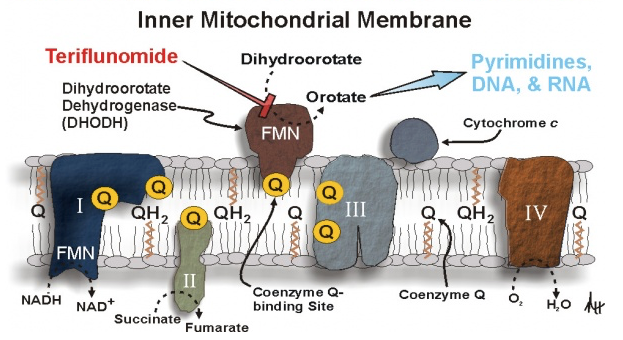
\includegraphics[width=0.7\linewidth]{Pictures/inhibition}
	\caption{}
	\label{fig:inhibition}
\end{figure}


p53 is considered a master regulator of proliferation, apoptosis, and has been linked to cell differentiation in a vareity of cell types. The effect of p53 has been explored in Treacher-Collins syndrome, another craniofacial disoder. Tcof1 mutations led to an increase in p53 levels in the neuroepithelium in mouse embryos. Knock-out of Trp53 in the TCS mouse model amerliorated the craniofacial abnormalitles. Additionally, p53 has shown to be involved in neural crest development. Stabilization of p53 protein resulted in fewer migrating CNC cells and in craniofacial defects in chick and mouse embryos, showing that p53 coordinates CNC cell growth by affecting cell cycle gene expression and proliferation at discrete developmental stages. These observations indicate that DHODH LOF may cause p53 up-regulation during embryonic development. 



\paragraph{Craniofacial and limb development}
~\\The primary phenotype associated with MS diagnosis is defective craniofacial and limb skeleton development. Skeletal development begins when loose networks of mesenchymal cells coalesce and condense, prefiguring mature cartilage and bone. Different mesenchymal populations give rise to anatomically distinct groups of bones. Neural crest-derived mesenchyme forms bones in the face, jaw and rostral calvarium whereas mesoderm-derived mesenchyme forms bones in the caudal calvarium, vertebral column, rib cage, and limbs. Osteoblasts differentiation is triggered by a variety of intra- and extracellular osteogenic signals, and  requires regulation by several transcription factors. Among these, the transcription factors Runx2 and Osterix/SP7 have critical roles in osteogenesis. 
~\\Previously, MC3T3-E1 cells had been used to show that depletion of DHODH activity decreased osteogenic gene expression. Expression and protein levels of p53 showed an increase in this study, however its relation to osteoblast differentiation was not explored. MC3T3-E1 cells contains Osx/SP7. Conditional inactivation of Osx/SP7 in cranial neural crest cells of mice has shown defects in craniofacial bone development. Additionally, a human patient with a homozygous mutation in Osx/SP7 displayed craniofacial and limb bone deformities suggesting roles of Osx/SP7 in bone differentiation and patterning during embryonic development. p53 is able to exert a repressive effect on Osx/SP7 leading to disruption in osteoblast differentiation. p53 

\textit{Osx} mRNA levels show significant up-regulation between E11.5 and E13.5 during mouse embryonic development, subsequent to the increased \textit{Dhodh} expression observed at E10.5. Therefore one of the mechanisms by which DHODH LOF may cause the MS phenotype is by inhibiting  Osx/SP7  due to an increase in p53  during craniofacial and limb development.


\paragraph{Animal model for Miller's syndrome}


\section{Summary and Aims}

\paragraph{Proposed mechanism}


\paragraph{Aim 1:} Using CRISPR-Cas9 genome editing to generate a mouse model for Miller's Syndrome
\paragraph{Aim 2:} Using western blotting and quantitative RT-PCR, determine if Trp53 levels are increased in mouse model during craniofacial and limb development 
\paragraph{Aim:} Using x, determine Trp53 localisation 
\paragraph{Aim 3:} Using x, determine if Osx is being inhibited due to increased Trp53 levels in mouse model 

\

\section{Generation of Miller's syndrome mouse model}

\paragraph{Genotyping}
\paragraph{Skeletal analysis}
\paragraph{Enzymatic assay}

\subsection{Predicted outcome}\

\section{p53 levels in Mouse model}

\subsection{Predicted outcome}
%\section{Determine if Trp53 levels are increased during mouse craniofacial and limb development as a result of DHODH LOF}














\end{document}